\chapter{Aplicaciones a los Baricentros de Wasserstein}\label{chap:app-bar-wass}

En este capítulo se presenta el tema principal de la tesis: la implementación del Descenso del Gradiente Estocástico en el Espacio de Wasserstein (SGDW), y su aplicación a la estimación del Baricentro de Wasserstein Bayesiano (BWB).

Para ello, se empieza explicando la implementación del SGDW, y se realizan experimentos con alguos muestreadores de distribuciones. Luego, se propone una adaptación del SGDW, donde se proyecta el baricentro sobre alguna variedad $\Manifold$ de medidas para que se vea más natural y atractivo. Finalmente, se utilizan estas implementaciones para el cálculo del BWB, donde se propone una técnica para poder estimarlo utilizando una GAN como prior.

\section{Implementación del SGDW}\label{sec:sgdw}  % MARK: SGDW

\RED[inline]{Revisar este párrafo reu 02/07}

En esta sección se presenta la implementación del SGDW. Se empieza explicando cómo se interpreta una imagen como una medida. Luego, se presentan las ligeras modificaciones al algoritmo original para que se pueda trabajar con medidas discretas. Posteriormente, se presentan los experimentos realizados con distintas medidas, y se discuten los resultados obtenidos.

\subsection{Interpretación de una Imagen como Medida}\label{ssec:interpr-imagen-medida}  % MARK: - Interpretación de una Imagen como Medida

Recordar que si $\mu\in \ProbSpace[\cX] $ es una medida discreta, entonces esta queda definida de la siguiente forma:
\begin{equation}\label{eq:medida-discreta}
    \mu = \sum_{i=1}^{n} m_i \delta_{x_i},
\end{equation}
donde $m \in \Simplex[n]$ es un vector de probabilidad en el Simplex y $ \left\{ x_1, \dots, x_n \right\} \subseteq \cX $ son sus posiciones.

En el caso de una imagen, esta se puede interpretar como una medida discreta, si se define $\cX \eqdef \left\{ x_1, \dots, x_n \right\} \subseteq \R^2$ como las posiciones de los píxeles, con $n \eqdef n_1 \times n_2$; y $m \in \Simplex[n]$ como el vector de probabilidad representando las intensidades de los píxeles. En este caso, si se asume que el espacio de imágenes es el espacio de probabilidad $\ProbSpace[\cX] $, entonces las distribuciones que muestrean imágenes corresponderían a distribuciones en el espacio $\ProbSpace[\ProbSpace[\cX] ] $.

\RED[inline]{Revisar este párrafo reu 02/07}
Las distribuciones que provienen de una imagen se implementan de manera eficiente tanto en tiempo y en memoria, utilizando su matriz de escala de grises. En la Figura~\ref{fig:face-example} se muestra un ejemplo de una distribución que proviene de una imagen, donde se presenta la imagen y su histograma para $n=1000$ muestras.

\begin{figure}[htbp]
    \centering
    
\includegraphics[height=6cm]{img/distr_draw/face_distrib.pdf}
    \hspace{2cm}
    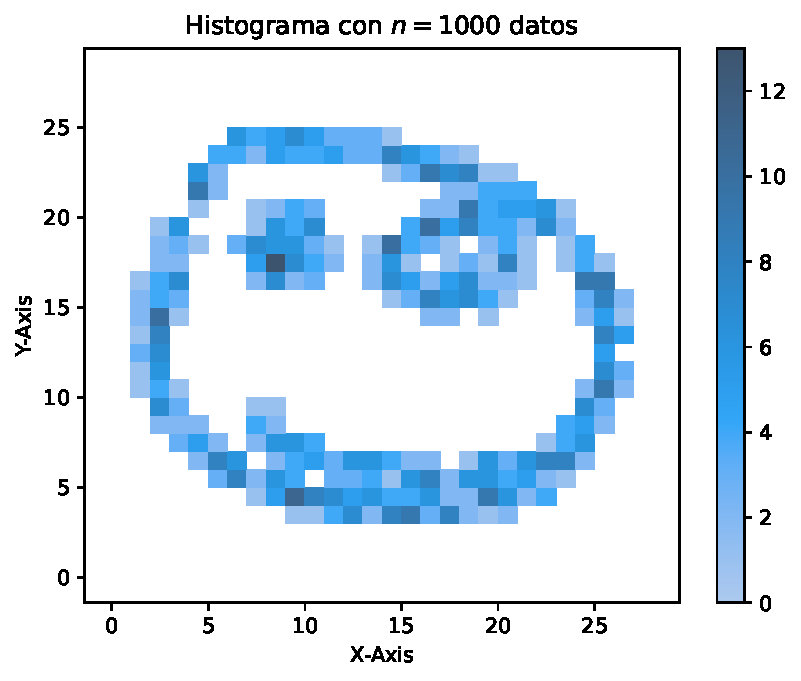
\includegraphics[height=6cm]{img/distr_draw/face_hist.pdf}
    \caption{A la izquierda, una imagen del dibujo de una cara. A la derecha, un histograma de $n=1000$ muestras obtenidas a partir de esta imagen.}
    \label{fig:face-example}
\end{figure}

\subsection{Implementación del Algoritmo}\label{ssec:implementacion-algoritmo}  % MARK: - Implementación del Algoritmo

Dado que el Algoritmo~\ref{alg:sgdw-clasico} está diseñado para medidas absolutamente continuas, se reinterpreta este algoritmo para que se pueda trabajar con medidas discretas. Para ello, se destaca que la Definición~\ref{def:sgdw} se puede reinterpretar como la $\eta_k$-interpolación geodésica entre las medidas $\mu_k$ y $\tilde \mu_k$, mientras que la Definición~\ref{def:bsgdw} se puede reinterpretar como el baricentro de las medidas $\qty( \mu_k, \tilde\mu_k^{(1)}, \dots, \tilde\mu_k^{(S_k)} )$ con pesos $\qty(1-\eta_k, \frac{\eta_k}{S_k}, \dots, \frac{\eta_k}{S_k}) \in \Simplex[S_k+1]$. De este modo, el Algoritmo~\ref{alg:sgdw-clasico} se extiende de la siguiente manera:
\begin{algorithm}[H]
    \caption{SGDW General}
    \label{alg:sgdw-general}
    \begin{algorithmic}[1]
        \Require Acceso a las muestras de $\Gamma(\dd \mu) \in \ProbSpace[\ProbSpace]$, un esquema de paso $(\eta_k)_k \in [0, 1]^\N$ y un esquema de paso $(S_k)_k \in \N^\N$.
        \State{$k\gets0$}
        \State{Muestrear $\mu_0 \sim \Gamma$}
        \Repeat
        \State{Muestrear $\tilde \mu_k^{(1)}, \dots, \tilde \mu_k^{(S_k)} \simiid \Gamma$}
        \State{$\gamma\gets\qty(1-\eta_k, \frac{\eta_k}{S_k}, \dots, \frac{\eta_k}{S_k})$}
        \State Definir $\mu_k$ como el baricentro de $\qty( \mu_k, \tilde\mu_k^{(1)}, \dots, \tilde\mu_k^{(S_k)} )$ con pesos $\gamma$.
        \State{$k\gets k+1$}
        \Until{un criterio de detención ha sido alcanzado.}
        \State\Return $\mu_k$
    \end{algorithmic}
\end{algorithm}

\RED[inline]{Revisar este párrafo reu 02/07}
Se destaca que en el Algoritmo~\ref{alg:sgdw-general} se mantiene la versión de la secuencia por lotes. Esto es debido para mantener una mayor generalidad, pues el caso original del Algoritmo~\ref{alg:sgdw-clasico} se recupera considerando $S_k=1,\ \forall k\in\N$.

\RED[inline]{Hay que revisar esta sección para ver cómo se pueden combinar o modificar.}

Como se está trabajando con imágenes, se puede aprovechar su estructura para calcular una estimación de los baricentros de manera más eficiente, utilizando el algoritmo de Baricentros de Wasserstein Convolucionales \cite{solomon2015convolutional} o su versión Insesgada (\textit{Debiased} en inglés) \cite{janati2020debiased}. Sin embargo, el Algoritmo~\ref{alg:sgdw-general} es lo suficientemente general para ser aplicado a cualquier medida discreta, utilizando por ejemplo, la estimación del algoritmo de Sinkhorn \cite{cuturi2013sinkhorn}.

Todos estos métodos de cálculo de baricentros se implementan de manera eficiente utilizando la librería de \textit{Python Optimal Transport} (POT) \cite{flamary2021pot}, donde además esta librería admite la paralelización de los cálculos por medio de la computación de Propósito General en Unidades de Procesamiento Gráfico (GPGPU por sus siglas en inglés) \cite{owens2008gpu}. En la implementación, se mantienen las versiones tanto para imágenes como para medidas discretas genéricas, para mayor generalidad y versatilidad.

\subsection{Experimentos con distintas medidas}\label{ssec:muestreando-gamma}  % MARK: - Muestreando de la Medida Gamma


Se considera una medida de referencia $\Prob_X \in \ProbSpace[\ProbSpace[\cX]]$ que corresponde a la forma ideal\FM{Con esto me esto refiriendo que no se utiliza directamente el data set, si no más bien una versión teórica y continua del mismo, donde nosotros tenemos acceso a esa variedad a través de muestras, y que la utilizamos como una aproximación de dicha variedad.} del conjunto de datos \textit{Quick, Draw!} \cite{jongejan2016quick}. Se desea calcular el baricentro de esta medida, utilizando el Algoritmo~\ref{alg:sgdw-general}. Para ello, se obtendrán dos aproximaciones. La primera, es la empírica:
\begin{equation}
    \hat \Prob_X = \frac{1}{N} \sum_{i=1}^{N} \delta_{\mu_i},
\end{equation}
donde $\left\{ \mu_i \right\}_{i=1}^{N} \subseteq \ProbSpace[\cX] $ es el conjunto de datos obtenido de la Sección~\ref{ssec:preparacion-dataset}, y $N$ es el tamaño del conjunto de datos. La segunda, es la medida generada por la WGAN $G_\theta : \cZ \to \ProbSpace[\cX]$, entrenada como se explica en el Capítulo~\ref{chap:WAE-WGAN}:
\begin{equation}
    \tilde \Prob_X
    = \pf{G_\theta} \Prob_Z
    %\int_{\cZ} \delta_{G_\theta(z)} (\dd \mu) \; \Prob_Z(\dd z),
\end{equation}
donde $\Prob_Z$ es la medida del espacio latente (en este caso, una distribución normal estándar).

Como ambas son estimaciones de la medida de referencia $\Prob_X$, se espera que el baricentro de estas medidas sean similares entre sí.

\subsection{Resultados y Discusión}\label{ssec:sgdw-resultados-discusion}  % MARK: -- Resultados y Discusión

\FM[inline]{En esta sección se podría incluir el cálculo de un baricentro, tanto del dataset como de la GAN}

\subsection{Conclusiones}\label{ssec:sgdw-conclusiones}  % MARK: -- Conclusiones

\FM[inline]{Insertar aquí alguna conclusión}

\FM[inline]{Una conclusión que se me ocurre es como los dos baricentros, el del conjunto de datos y el de la GAN se parecen, algo que debería de pasar puesto que ambos están aproximando a alguna medida de referencia $\Prob_X$}


% \newpage
\section{SGDW Proyectado}\label{sec:sgdwp}  % MARK: - Section SGDWP

% \newpage
\section{Baricentro de Wasserstein Bayesiano}\label{sec:bwb}  % MARK: - Section Baricentro de Wasserstein Bayesiano


Teniendo un conjunto de modelos finito, dígase, $\Models \subseteq \ProbSpace[\cX] $ con $| \Models | = N < + \infty$, un acercamiento ``ingenuo'' para calcular la medida posterior sobre este espacio debría considerar el vector de verosimilitudes $L_n = (\cL_n(\mu))_{\mu \in \Models} \in \R^N$. El problema con este enfoque es que, por definición, es bastante probable que uno de los puntos en que se evalúa $\rho_\mu$ sea $0$. Es decir, si $\exists x_i \in D \colon \rho_\mu(x_i) = 0$, entonces ese modelo tendrá una verosimilitud nula. En la práctica, esto sucede con mucha frecuencia. Por este motivo, se decide tomar otro enfoque.


\subsection{Construcción de la Posterior Usando una GAN}\label{ssec:construccion-posterior}  % MARK: - Construcción de la Posterior Usando una GAN

\RED[inline]{Hay que seguir revisando esta sección}

Como se explicó en secciones anteriores,\FM{Aquí sería bueno incluir las secciones de lo que se habla esto, sguramente el de la GAN y WGAN}
dada una medida de referencia $\Prob_X$\footnote{del cuál se tiene acceso a través de una muestra para obtener una medida empírica $\hat\Prob_X = \frac{1}{N}\sum_{i=1}^{N} \delta_{x_i}$}\FM{Corregir} lo que hacen las redes generativas es aproximarla por medio de un modelo generativo $\Prob_G$. Gracias a esta propiedad, se propone utilizar una GAN como prior para poder calcular la posterior. Cabe destacar que, a pesar de que la idea de utilizar una GAN como prior fue original, ya existía un trabajo que propone algo similar \cite{patel2019bayesian}, sin embargo, en este trabajo de tesis se formalizan estas ideas.

Dada una red generadora $G_\theta \colon \cZ \to \ProbSpace[\cX] $ con una medida en el espacio latente $\Prob_Z$, se propone utilizar como prior a la medida
\begin{equation}
    \Pi^G \eqdef \pf{G_\theta} \Prob_Z.
\end{equation}
De esta manera, la posterior tendría la siguiente forma:
\begin{equation}
    \Pi_n(\dd \mu)
    \eqdef \frac{\cL_n(\mu)}{\int_{\ProbSpace[\cX]} \cL_n(\nu) \; \Pi^G(\dd \nu)} \; \Pi^G(\dd \mu)
    = C^{-1} \cL_n(\mu) \; \Pi^G(\dd \mu),
\end{equation}
donde $C \eqdef \int_{\ProbSpace[\cX]} \cL_n(\nu) \; \Pi^G(\dd \nu)$ es una constante de normalización.

Dada alguna función arbitraria $\Pi_n$-integrable $g$ (como por ejemplo $\mu \mapsto \Wasserstein[p]{\mu}{\nu}^p$), se puede comprobar lo siguiente:
\begin{align}
     & \int_{\ProbSpace[\cX]} g(\mu) \; \Pi_n(\dd \mu)                         \\
     & = C^{-1} \int_{\ProbSpace[\cX]} g(\mu) \cL_n(\mu) \; \Pi^G(\dd \mu)     \\
     & = C^{-1} \int_{\cZ} g(G_\theta(z)) \cL_n(G_\theta(z)) \; \Prob_Z(\dd z) \\
     & = \int_{\cZ} g(G_\theta(z)) \; \Pi^Z_n(\dd z),
\end{align}
donde $\Pi^Z_n(\dd z)$ es la \textit{medida posterior en el espacio latente} y se define por
\begin{equation}
    \Pi^Z_n(\dd z) \eqdef C^{-1} \cL_n(G_\theta(z)) \; \Prob_Z(\dd z).
\end{equation}

Por la Definición~\ref{def:operador-push-forward} del operador push-forward, se concluye la siguiente propiedad de la medida posterior:
\begin{equation}\label{eq:posterior-en-latente}
    \Pi_n = \pf{G_\theta} \Pi^Z_n.
\end{equation}
La forma de interpretar la ecuación~\eqref{eq:posterior-en-latente} es que para obtener un muestreo de la posterior $\Pi_n(\dd \mu)$ basta con hacer un muestreo de la posterior en el espacio latente $\Pi^Z_n(\dd z)$ y después aplicar la red generadora $G_\theta$.

Esto resulta beneficioso, pues delega la tarea de muestrear a partir de la posterior al espacio latente $\cZ$ (el cuál, en la práctica, es $\R^{d_z}$), la cual es mucho más fácil de simular. Por ejemplo, una manera de obtener muestreos a partir de $\Pi^Z_n$, es por medio del método de Markov Chain Monte Carlo (MCMC) \cite{andrieu2003introduction,brooks2011handbook,goodman2010ensemble}.\RED{Revisar este párrafo}






% Esto es, dado una red generadora $G_\theta \colon \cZ \to \ProbSpace[\cX] $, se propone como prior sobre el conjunto de modelos de la siguiente manera:
% \begin{equation}
%     \Pi_G(\dd \mu) \eqdef \pf{G_\theta} \Prob_Z(\dd \mu).
% \end{equation}
% De manera que la posterior tendría la siguiente forma:
% \begin{equation}
%     \Pi_n(\dd \mu)
%     \eqdef \frac{\cL_n(\mu)}{\int_{\ProbSpace[\cX]} \cL_n(\nu) \Pi_G(\dd \nu)} \Pi_G(\dd \mu)
%     = \frac{1}{C} \cL_n(\mu) \Pi_G(\dd \mu),
% \end{equation}
% donde $C \eqdef \int_{\ProbSpace[\cX]} \cL_n(\nu) \Pi_G(\dd \nu)$ es una constante de normalización.


% De este modo, la función valor del problema de optimización de la Definición~\ref{def:baricentroWassersteinBayesiano} se puede reescribir de la siguiente manera:
% \begin{align}
%      & \int_{\ProbSpace[\cX]} \Wasserstein[p]{\mu}{\nu}^p \; \Pi_n(\dd \nu)                              \\
%      & = \frac{1}{C} \int_{\ProbSpace[\cX]} \Wasserstein[p]{\mu}{\nu}^p \cL_n(\nu) \; \Pi_G(\dd \mu)     \\
%      & = \frac{1}{C} \int_{\cZ} \Wasserstein[p]{\mu}{G_\theta(z)}^p \cL_n(G_\theta(z)) \; \Prob_Z(\dd z)
% \end{align}

% Con este enfoque, notamos que la función de probabilidad de densidad de la medida posterior en el espacio latente es:
% \begin{equation}
%     \Pi_n^Z (\dz) \eqdef \frac{1}{C} \cL_n(G_\theta(z)) \; \Prob_Z(\dz).
% \end{equation}
% Y de este modo, la medida posterior en el espacio de los modelos es:

% El objetivo de obtener esta función de distribución, es que nos dice que podemos simular muestras de la posterior $\Pi_n(\dd \mu)$ a través de la red generativa $G_\theta$. En efecto, basta darse cuenta que






\subsection{Resultados y Discusión}\label{ssec:bwb-resultados-discusion}  % MARK: - Resultados y Discusión

\subsection{Conclusiones}\label{ssec:bwb-conclusiones}  % MARK: - Conclusiones

